%%% Reusable Start
\documentclass[a4paper,4pt]{article}
\usepackage[UTF8]{ctex}
\usepackage{geometry}
\usepackage{titlesec}
\usepackage{indentfirst}
\usepackage{graphicx} %use graph format
\usepackage{subfigure}
\usepackage{epstopdf}
\usepackage{hyperref}
\usepackage{float}
\usepackage{amsmath}
\usepackage{amssymb}
\usepackage{multirow}
\usepackage{array}
\usepackage{enumerate}
\usepackage{enumitem} 
\usepackage{bookmark}
\usepackage{booktabs}
\usepackage{multirow}
\usepackage{bigstrut}
\usepackage[backend=bibtex]{biblatex}
\usepackage{pgfplots}
\usepackage{pgfplotstable}
\usepackage{siunitx}
\usepackage{datetime}
%插入中文日期
\renewcommand{\today}{\number\year 年 \number\month 月 \number\day 日}
%% for inserting code
\usepackage{listings}
\usepackage{xcolor}
\definecolor{mygreen}{rgb}{0.3,0.7,0}  
\definecolor{mygray}{rgb}{0.5,0.5,0.5}  
\definecolor{myblue}{rgb}{0.4,0.7,1}
\definecolor{mywhite}{rgb}{0.9,0.9,0.9}
\definecolor{mymauve}{rgb}{0.58,0,0.82}
\definecolor{mybackcolor}{RGB}{62,62,62}
\definecolor{myIdt}{rgb}{0.8,0.6,1}
\lstset{ %  
  backgroundcolor=\color{mybackcolor},   % choose the background color; you must add \usepackage{color} or \usepackage{xcolor}  
  basicstyle=\small\ttfamily\color{mywhite},        % the size of the fonts that are used for the code  
  breakatwhitespace=false,         % sets if automatic breaks should only happen at whitespace  
	breaklines=true,                 % sets automatic line breaking  
  captionpos=bl,                    % sets the caption-position to bottom  
  commentstyle=\color{mygreen},    % comment style  
  %deletekeywords={...},            % if you want to delete keywords from the given language  
  escapeinside={\%*}{*)},          % if you want to add LaTeX within your code  
  extendedchars=true,              % lets you use non-ASCII characters; for 8-bits encodings only, does not work with UTF-8  
  %frame=single,                    % adds a frame around the code  
  keepspaces=true,                 % keeps spaces in text, useful for keeping indentation of code (possibly needs columns=flexible)  
  keywordstyle=\color{myblue},       % keyword style  
  %language=Python,                 % the language of the code  
  morekeywords={*,...},            % if you want to add more keywords to the set  
  numbers=left,                    % where to put the line-numbers; possible values are (none, left, right)  
  numbersep=-15pt,                   % how far the line-numbers are from the code  
  numberstyle=\small\color{mygray}\ttfamily, % the style that is used for the line-numbers  
  rulecolor=\color{black},         % if not set, the frame-color may be changed on line-breaks within not-black text (e.g. comments (green here))  
  showspaces=false,                % show spaces everywhere adding particular underscores; it overrides 'showstringspaces'  
  showstringspaces=false,          % underline spaces within strings only  
  showtabs=false,                  % show tabs within strings adding particular underscores  
  stepnumber=1,                    % the step between two line-numbers. If it's 1, each line will be numbered  
  stringstyle=\color{orange},     % string literal style  
  tabsize=2,                       % sets default tabsize to 2 spaces  
  %title=myPython.py                   % show the filename of files included with \lstinputlisting; also try caption instead of title  
	rulesepcolor=\color{red!20!green!20!blue!20},
	identifierstyle=\color{myIdt},
	} 
%% end of code style



\begin{document}

%第二种封面
\begin{titlepage}
  \heiti
  \vspace*{20pt}
  \begin{center}
    \fontsize{20pt}{0} {清华大学第三届人工智能挑战赛}\\
    \vspace*{20pt}
    \fontsize{20pt}{0} \textbf{清华大学自动化系第十八届新生C语言大赛}\\
    \vspace*{20pt}
    \fontsize{20pt}{0} \textbf{参赛手册(\today)}\\
    \vspace*{280pt}
    \normalsize
    \rmfamily
    \begin{tabular}{c} %表格,lr表示左对齐|右对齐
      \textbf{指导单位}            \\
      共青团清华大学委员会         \\
      清华大学学生科学技术协会     \\
      共青团清华大学自动化系委员会 \\
      \\
      \textbf{承办单位}            \\
      清华大学自动化系学生科协     \\
      \\
      \textbf{大赛官网}            \\
      https://www.thuasta.cn       \\
    \end{tabular}
  \end{center}
\end{titlepage}


\tableofcontents%目录
\newpage%换页
\section{概述}
FC18为四方势力在地图上进行回合制对战的策略游戏,玩家需要力求攻占其他玩家的防御塔、占领尽可能大的领地、消灭或俘虏其他玩家的兵团以获得胜利。每个玩家需要编写AI,根据裁判程序提供的场地信息,决策己方势力在该回合的行动,并返回给裁判程序,以控制己方的行为。\par
作为塔防游戏,每个势力在开始时各在一角的区域内拥有一座防御塔,防御塔周围的一定区域是自己的领地。玩家需要利用防御塔的生产力,完成生产兵团或升级防御塔的任务。生产出的作战兵团可以在场上移动,攻击其他势力的防御塔或兵团(减少他们的生命值);生产出的工程兵团则可以修改地形、修理防御塔(恢复防御塔的生命值)、新建新的防御塔。选手各自操控防御塔和兵团,击杀敌方的防御塔或兵团,同时应尽可能建造防御塔,占领尽可能大的地盘。\par


\begin{figure}[htbp]   %用htbp表示插入位置自动排版
  \centering
  \includegraphics[width=5.5 in]{example.png}
  \caption{游戏场地示意图}
  \label{jpg:示例图片1}
\end{figure}

\subsection{样例AI和最新规则}

最新的比赛规则在 https://github.com/HelinXu/FC18\_handbook 。其中包括了选手对于规则疑问的Q\&A。\par
样例AI在 https://github.com/HelinXu/FC18\_player\_code\_sample 。这个样例AI可以帮助选手快速入门比赛。\par


\section{游戏规则}
游戏中有以下角色:防御塔,作战兵团(分为战士、弓箭手、法师),工程兵团(分为建设者、开拓者)。\par
游戏中角色的基本操作包括:运动(塔不可以运动,各种兵团均可运动),进攻(塔进攻兵团,作战兵团进攻兵团,作战兵团进攻塔),建设(塔生产各种兵团/升级自身,工程兵团-建设者修改地形,工程兵团-建设者修复塔,工程兵团-开拓者新建防御塔)。
\begin{enumerate}[fullwidth, itemindent=2em, label=(\arabic*)]
  \item 场地和地形:在 15 * 15 的方格地图上,分布了平原、山地、森林、沼泽、道路五种地形。四方势力在场地上修建防御塔、生产并操作若干种兵团。
  \item 防御塔:共分8级,具有生命值、战斗力属性,能生产己方兵团、攻击敌方兵团。防御塔的等级越高,就会拥有更高的生产力、战斗力、生命值;如果防御塔内有己方兵团驻扎,则防御塔的战斗力会更强。
  \item 作战兵团:分为战士、弓箭手、法师三种,具有行动力、战斗力、生命值属性,能移动、攻击敌方兵团或防御塔。
  \item 工程兵团:分为建设者和开拓者。建设者具有行动力和劳动力属性,可以移动、修复己方防御塔或修改地形;开拓者具有行动力,可以移动并建立新的防御塔。
  \item 计分规则:选手各自操控防御塔和兵团,建造防御塔,摧毁敌方的防御塔。在游戏结束时,得分正比于己方防御塔占领的领地大小。
\end{enumerate}
\par

\subsection{防御塔}
每个势力最初时拥有1座防御塔,最多拥有10座防御塔。当某势力没有防御塔时,该势力将被判为失败。
每座防御塔周围地图会附加己方的占有属性值,该属性值见表\ref{领地};在某一方格上占有值最高的一方会占领该领地。游戏的目的是通过修建防御塔,占领尽可能大的领地,从而获得分数。
\begin{figure}[htbp]   %用htbp表示插入位置自动排版
  \centering
  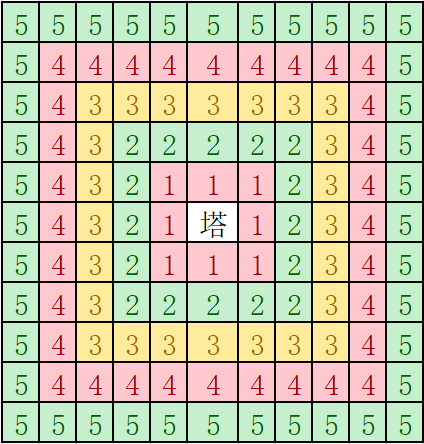
\includegraphics[width=2.5 in]{距离.png}
  \caption{距离计算示意图}
  \label{jpg:示例图片2}
\end{figure}

% Table generated by Excel2LaTeX from sheet 'Sheet1'
\begin{table}[htbp]
  \centering
  \caption{防御塔周围领地占有值}
  \begin{tabular}{c|c|c|c|c|c|c|c}
    \hline
    距防御塔距离d  & 0     & 1   & 2  & 3  & 4  & 5  & 6+ \bigstrut \\
    \hline
    施加占有属性值 & $inf$ & 100 & 80 & 50 & 20 & 10 & 0 \bigstrut  \\
    \hline
  \end{tabular}%
  \label{领地}%
\end{table}%

防御塔有以下属性:
\begin{enumerate}[fullwidth, itemindent=2em, label=(\arabic*)]
  \item 所属玩家ID。
  \item 等级$N$。等级越高,相关属性越好。具体的数据如表\ref{塔等级表}所示。
  \item 生产力$W_N$。为每回合可用的生产力,可用于生产战士、弓箭手、法师、建设者、开拓者,或升级防御塔自身。具体见表\ref{塔生产}。如果上一回合塔选择了生产,但未完成该生产任务,本回合选择攻击,则上一回合的生产进度会被保留,这样在下一回合假如继续添加生产该任务的命令,会在上一回合基础上继续生产。若防御塔的某个生产任务尚未完成,玩家又指定了新任务,则未完成的生产任务的完成度将被保留。
  \item 等级生命值上限$HP_N$,当前生命值$hp$。等级生命值上限$HP_N$仅与等级正相关,实际生命值$hp$会受到进攻而减小,由于建设者的维护而增加。实际生命值$hp$与等级生命值上限$HP_N$的比值决定了实际战斗力,实际生命值较弱的塔的实际战斗力也很弱。当实际生命力 $hp$ 被进攻方降低至0以下时,我方丧失该塔,塔等级下降4级:等级下降后,若不足1级,则塔消失,该单位恢复原来地形;若塔尚存在,则降级后的塔主权归对方所有(塔被俘虏)。同时,塔所在方格的所有敌方兵团(不允许兵团进入别人塔所在方格,因此塔中所有兵团都是本塔方的兵团),都直接杀死。
  \item 等级战斗力$F_N$,实际战斗力$f$。实际战斗力$f$正比于$F_N$,正比于相对生命值$\frac{hp}{HP_N}$,并会额外附加兵团驻扎情况带来战斗力增益$f_c$(具体增益规则如表\ref{兵团}所示)。
  \item 攻击距离$d_c$。
\end{enumerate}
\par

你可以为防御塔添加生产或攻击命令。


\subsection{作战兵团}
在同一个时间,同一个地图方格(防御塔所在方格除外)内的作战兵团、工程兵团数量各自不能超过1个。作战兵团受到攻击时,生命值减少直至兵团死亡;工程兵团受到攻击时,会直接被对方俘虏。\par
兵团有三个种类:战士(近战单位)、弓箭手(远程单位)、法师(高级进攻单位)。
其中,弓箭手可以远程轰炸其他单位且自身不受伤害。法师具有较高的移动力。\par
作战兵团有以下属性:
\begin{enumerate}[fullwidth, itemindent=2em, label=(\arabic*)]
  \item 行动力$M_c$。具体见表\ref{兵团}。兵团从一个单元格移动到另一个相邻单元格(即上下左右四个方向)将消耗一定行动力,地形和行动力共同决定一回合中,一个兵团能运动多远。
  \item 满血战斗力$F_c$,实际战斗力$f$。与塔类似。
  \item 生命值上限$HP_c$,当前生命值$hp$。与塔类似。
  \item 攻击距离$d_c$。兵团只能攻击在攻击范围内的对象。
  \item 所属玩家ID。
\end{enumerate}
\par
作战兵团能进行的操作有:在地图上移动、对敌方军团发起进攻、对敌方防御塔发起进攻。


\subsection{工程兵团}
工程兵团分为:建设者、开拓者。工程兵团所处单元格没有己方作战兵团护卫时,任何敌方作战兵团对其的进攻操作,会直接将其俘虏。\par

\subsubsection{建设者}
开拓者有关参数为行动力$M_c$(同作战兵团),劳动力$B$和玩家所属ID。其中,劳动力$B$是建设者特有的属性值。建设者的劳动力大小初始值为3,表示其能进行三次工程建造。\par %TODO
建设者可以进行地形修改(只能实现平原-森林的互换)和防御塔维修(单次修理将恢复防御塔该等级最大生命值的1/3(向下取整))两种操作,两种操作各自需要1点劳动力消耗。发起操作时,建设者必须先运动到对应方格上。
\subsubsection{开拓者}
开拓者有关参数为行动力$M_c$和玩家所属ID。\par
已有的防御塔每次生产一个开拓者,等级下降1(本来为1则不再下降),开拓者可以在己方领地上一次性地建造一座新的防御塔建造。注意:必须运动到己方领地才能建造,且建造后开拓者即消失。




\section{你需要做什么}
\subsection{概述}
所有玩家的AI都可以从\texttt{Info}中读取当前场上各方势力的兵团、防御塔的信息,并设计算法,并按照统一的接口\texttt{CommandList}给裁判程序回传命令,操控己方势力;在游戏中,选手只需要在\texttt{ai.cpp}文件中的\texttt{void player\_ai(Info\& info) \{ \   \}}函数中填写自己的代码,并最终只需要提交\texttt{ai.cpp}文件。

\subsection{玩家添加命令示例}
玩家每回合给防御塔和兵团添加的命令总数量不得超过50个,超出数量限制的命令会被忽略。另外规定:防御塔最多10座,作战兵团最多10个,工程兵团最多10个。如果己方兵团已经有10个,此时俘虏了一个敌方兵团,则敌方兵团直接消失,而不是转换为我方兵团。防御塔同理。
\subsubsection{防御塔}
\begin{lstlisting}[language={C++}]  %插入代码块
      
      info.myCommandList.addCommmand(towerCommand, {TAttackCorps, 本防御塔ID, 目标兵团ID})  //防御塔攻击兵团
      info.myCommandList.addCommmand(towerCommand, {TProduct, 本防御塔ID, 生产任务类型(见下方枚举类型)})  //防御塔设定生产任务
\end{lstlisting}
说明:单个回合中,对每座防御塔,只能添加一个命令。多余命令会被忽略。

\subsubsection{作战兵团}
\begin{lstlisting}[language={C++}]  %插入代码块
      
      info.myCommandList.addCommmand(corpsCommand, {CMove, 本兵团ID, 方向(Cup / Cdown / Cleft / Cright)})  //移动
      info.myCommandList.addCommmand(corpsCommand, {CAttackCorps, 本兵团ID, 目标兵团ID})  //兵团攻击兵团
      info.myCommandList.addCommmand(corpsCommand, {CAttackTower, 本兵团ID, 目标防御塔ID})  //兵团攻击防御塔
\end{lstlisting}

说明:在单个回合中,对于单个作战兵团,仅能添加:若干移动指令(也可以不移动)+ 攻击命令(添加攻击命令需要还有剩余 >0 的行动力。如果移动命令完成后,行动力为 0,则该回合无法进攻。如果输入的命令无效,无效命令会被直接忽略。)

注意:若攻击命令有效,在发动攻击后兵团的行动力将被置为0,即本回合不能再进行其他操作。任何兵团处在己方势力塔的方格上即视为驻扎在塔内,只有当离开该方格才视为退出驻扎。\par

移动命令无效的情形包括:
超出地图范围,
行动力为零,
目标方格存在对方势力(兵团和塔),
目标方格内己方兵团数量不符合要求。

\subsubsection{工程兵团:建设者}
\begin{lstlisting}[language={C++}]  %插入代码块
          
      info.myCommandList.addCommmand(corpsCommand, {CMove, 本兵团ID, 方向(Cup / Cdown / Cleft / Cright)})  //移动
      info.myCommandList.addCommmand(corpsCommand, {CRepair, 本兵团ID})  //修复防御塔
      info.myCommandList.addCommmand(corpsCommand, {CChangeTerrain, 本兵团ID, 目标地形(枚举类型)})  //修改地形
\end{lstlisting}
说明:仅支持地形“平原-森林”之间的相互转换。在单个回合中,对于单个建设者,仅能添加:若干移动指令(也可以不移动)+修复防御塔/修改地形(二选一。此时需要还有剩余>0的行动力。如果移动命令完成后,行动力为0,则该回合无法修复/修改。如果输入的命令无效,无效命令会被直接忽略。)修改地形需要在该回合结束之后统一起作用。

\subsubsection{工程兵团:开拓者}
\begin{lstlisting}[language={C++}]  %插入代码块
          
      info.myCommandList.addCommmand(corpsCommand, {CMove, 本兵团ID, 方向(Cup / Cdown / Cleft / Cright)})  //移动
      info.myCommandList.addCommmand(corpsCommand, { CBuild, 本兵团ID })  //建立新防御塔
\end{lstlisting}
说明:在单个回合中,对于单个开拓者,仅能添加:若干移动指令(也可以不移动)+建立新防御塔(此时需要还有剩余>0的行动力。如果移动命令完成后,行动力为0,则该回合无法新建防御塔。一旦执行了新建防御塔命令后,开拓者即消失。建立新防御塔的条件:该方格是己方领地,该方格尚未建立防御塔。)新建的防御塔需要从下一回合开始可以起作用。

%枚举
\section{计分规则}
在游戏进程中防御塔数量降为0的玩家,判定出局。第一位出局的玩家获得最低位次,第二位出局的玩家获得次低位次,依次类推。\par
当游戏进行至300回合(每个玩家都进行过300回合操作)后,场上还未出局的玩家将按照游戏结束时各自占领的领地大小,获得得分,进行排名。\par
在天梯上进行对决时,出现平局情况,双方并列,得分一致。但在复赛和决赛中,如果出现平局情况,则重新进行比赛,直到分出胜负。

\section{附录}
塔相关结算方法如下:
\begin{equation}
  f = F_N \cdot \frac{hp}{HP_N} + \Sigma f_b\label{f}
\end{equation}
兵团攻击塔时,生命值的结算方式如下:
\begin{equation}
  \begin{aligned}
    hp_{\text{塔}}   & \ -= & \ 30 \cdot k_c \cdot e^{0.04(f_{\text{兵}}-f_{\text{塔}})} & ;                       \\
    hp_{\text{兵团}} & \ -= & \ 28 \cdot e^{0.04(f_{\text{塔}}-f_{\text{兵}})}           & , \text{当兵团非弓箭手} \\
    hp_{\text{兵团}} & \ -= & \ 0                                                        & , \text{当兵团为弓箭手} \\
  \end{aligned}
  \label{hp1}
\end{equation}
塔只能攻击距离为2及以内的兵团。塔攻击兵团时,生命值的结算方式如下:
\begin{equation}
  \begin{aligned}
    hp_{\text{兵团}} & \ -=\ 30 \cdot e^{0.04(f_{\text{塔}}-f_{\text{兵}})}, \text{对于所有兵团种类} \\
    hp_{\text{塔}}   & \ -=\ 0                                                                       \\
  \end{aligned}
  \label{hp2}
\end{equation}
兵团相关结算方式如下:
\begin{equation}
  f = F_c \cdot \frac{hp}{HP_c} + f_t\label{f2}
\end{equation}
兵团只能攻击在攻击范围内的对象,不同兵团的攻击距离$d_c$如表\ref{兵团}所示。兵团B受到兵团A攻击时,生命值的结算方式如下:
\begin{equation}
  \begin{aligned}
    hp_{B} & \ -= & \ 30 \cdot e^{0.04(f_{A}-f_{B})} & ;                        \\
    hp_{A} & \ -= & \ 28 \cdot e^{0.04(f_{B}-f_{A})} & , \text{当兵团A非弓箭手} \\
    hp_{A} & \ -= & \ 0                              & , \text{当兵团A为弓箭手} \\
  \end{aligned}
  \label{hp2}
\end{equation}\par
请注意:攻击会对双方生命值造成损失,其中生命值弱的一方损失更大。如果攻击的发起者生命值更弱,则攻击发起者受到的损失很可能更大。

% Table generated by Excel2LaTeX from sheet 'Sheet1'
\begin{table}[htbp]
  \centering
  \caption{塔等级表}

  \begin{tabular}{c|c|c|c}
    \hline
    等级$N$ & 生产力$W_N$ & 等级战斗力$F_N$ & 等级生命力上限$HP_N$ \bigstrut \\
    \hline
    1       & 10          & 25              & 100 \bigstrut                  \\
    \hline
    2       & 15          & 27              & 110 \bigstrut                  \\
    \hline
    3       & 20          & 29              & 120 \bigstrut                  \\
    \hline
    4       & 25          & 32              & 130 \bigstrut                  \\
    \hline
    5       & 30          & 35              & 140 \bigstrut                  \\
    \hline
    6       & 35          & 38              & 150 \bigstrut                  \\
    \hline
    7       & 40          & 41              & 160 \bigstrut                  \\
    \hline
    8       & 45          & 45              & 170 \bigstrut                  \\
    \hline
  \end{tabular}%
  \label{塔等级表}%
\end{table}%


% Table generated by Excel2LaTeX from sheet 'Sheet1'
\begin{table}[htbp]
  \centering
  \caption{塔生产任务表}
  \begin{tabular}{c|c}
    \hline
    生产任务           & 所需的生产力值 \bigstrut \\
    \hline
    战士               & 40 \bigstrut             \\
    \hline
    弓箭手             & 60 \bigstrut             \\
    \hline
    法师               & 100 \bigstrut            \\
    \hline
    建设者             & 40 \bigstrut             \\
    \hline
    开拓者             & 40 \bigstrut             \\
    \hline
    升级(N升级到N+1) & N*40 \bigstrut           \\
    \hline
  \end{tabular}%
  \label{塔生产}%
\end{table}%

% Table generated by Excel2LaTeX from sheet 'Sheet1'
\begin{table}[htbp]
  \centering
  \caption{兵团参数表}
  \begin{tabular}{c|c|c|c|c|c}
    \hline
    兵种Crops           & 战士 & 弓箭手 & 法师 & 建设者 & 开拓者 \bigstrut \\
    \hline
    战斗力增益系数$f_c$ & 2    & 2      & 4    & NA     & NA \bigstrut     \\
    \hline
    攻城系数$k_c$       & 0.4  & 0.7    & 0.5  & NA     & NA \bigstrut     \\
    \hline
    攻击距离$d_c$       & 1    & 2      & 1    & NA     & NA \bigstrut     \\
    \hline
    行动力$M_c$         & 4    & 4      & 8    & 4      & 4 \bigstrut      \\
    \hline
    生命力上限$HP_c$    & 60   & 50     & 70   & NA     & NA \bigstrut     \\
    \hline
    满血战斗力$F_c$     & 36   & 30     & 44   & NA     & NA \bigstrut     \\
    \hline
    劳动力$B$           & NA   & NA     & NA   & 3      & NA \bigstrut     \\
    \hline
    $m\_BattleType$     & 0    & 1      & 2    & NA     & NA \bigstrut     \\
    \hline
    $m\_BuildType$      & NA   & NA     & NA   & 0      & 1 \bigstrut      \\
    \hline
  \end{tabular}%
  \label{兵团}%
\end{table}%

% Table generated by Excel2LaTeX from sheet 'Sheet1'
\begin{table}[htbp]
  \centering
  \caption{地形参数表}
  \begin{tabular}{c|c|c|c|c|c}
    \hline
    地形                & 平原 & 山地 & 森林 & 沼泽 & 道路 \bigstrut \\
    \hline
    地形战斗力增益$f_t$ & 0    & 5    & 3    & -3   & 0 \bigstrut    \\
    \hline
    地形行动力消耗$m_t$ & 2    & 4    & 3    & 4    & 1 \bigstrut    \\
    \hline
  \end{tabular}%
  \label{地形}%
\end{table}%



\end{document}